\section{Performance Evaluation}
\label{sec:pe}
%We consider a $5000 \times 5000 m^2$
%sparse sensing field with
%$100$ relay nodes.
The total number of relay nodes is $100$,
excluding $src$,
which means that $N=100$.
The Poisson-contact mobility model is synthetic,
%quasi-synthetic,
%in which
where the parameter $\lambda$ is set to
$4 \times 10^{-3}$ $s^{-1}$.
The source node is fixed at the center of the network scenario.
%The speed of nodes is randomly selected in a uniform distribution
%changing from 4 to 10 m/s,
%and the communication range of these nodes is set to be $20$$m$.
We set the parameter $\rho$ as $1.1 \times 10^{-2}$ $s^{-1}$.
The weight $\alpha$ is limited,
i.e., $\alpha \in (0, 1)$.
The minimum detection cycle is that $T_{m}=1$ $s$.
Note that all statistical results in the experiments
are obtained by repeating $20$ times.
%We consider two cases in the simulations.
%In the first case (Section~\ref{subsec:wo_detc}),
%we set $U(t)=0$,
%which means there is no selfish detection.
%In the second case (Section~\ref{subsec:full_detc}),
%we adopt the selfish detection method and
%keep detecting during whole lifetime of network.
%In each simulation,
%$M$ messages are created,
%whose maximal lifetime $T$ increases from $0$$s$ to $2000$$s$.

\subsection{Accuracy of Modeling}
\label{subsec:pe_valid}
\begin{figure}
  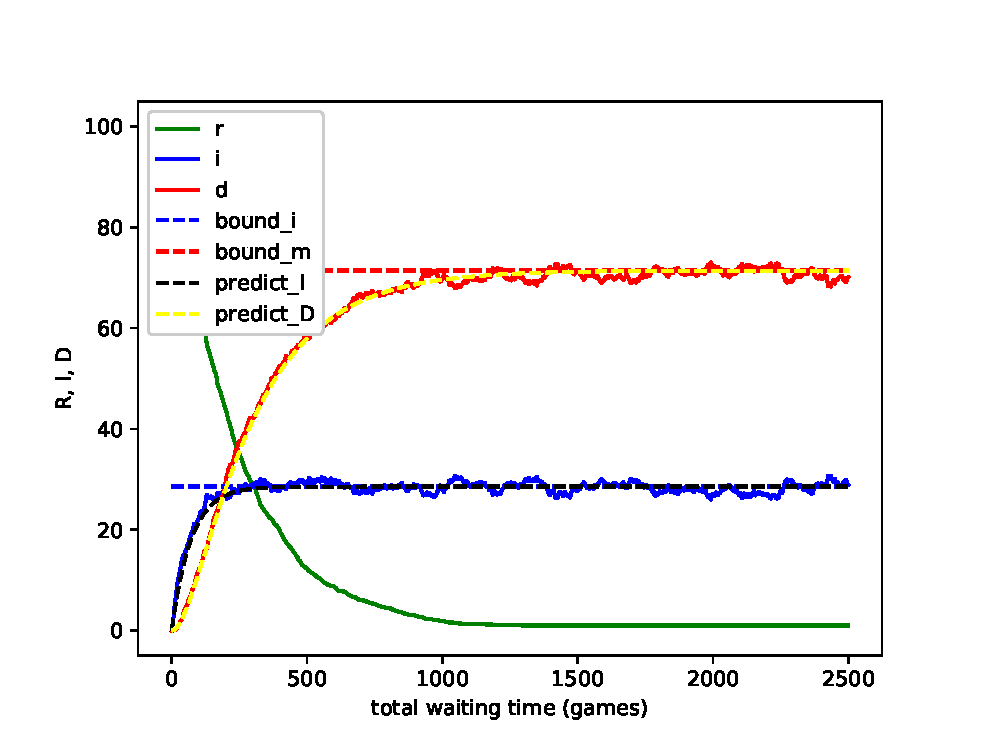
\includegraphics[width=.45\textwidth]{fig/twohop_without_detection.eps}
  \caption{Comparison of the theoretical and simulation results
  of the proposed ODE model in case $1$.}
  \label{fig:twohop_predict_wod}
\end{figure}
\begin{figure}
  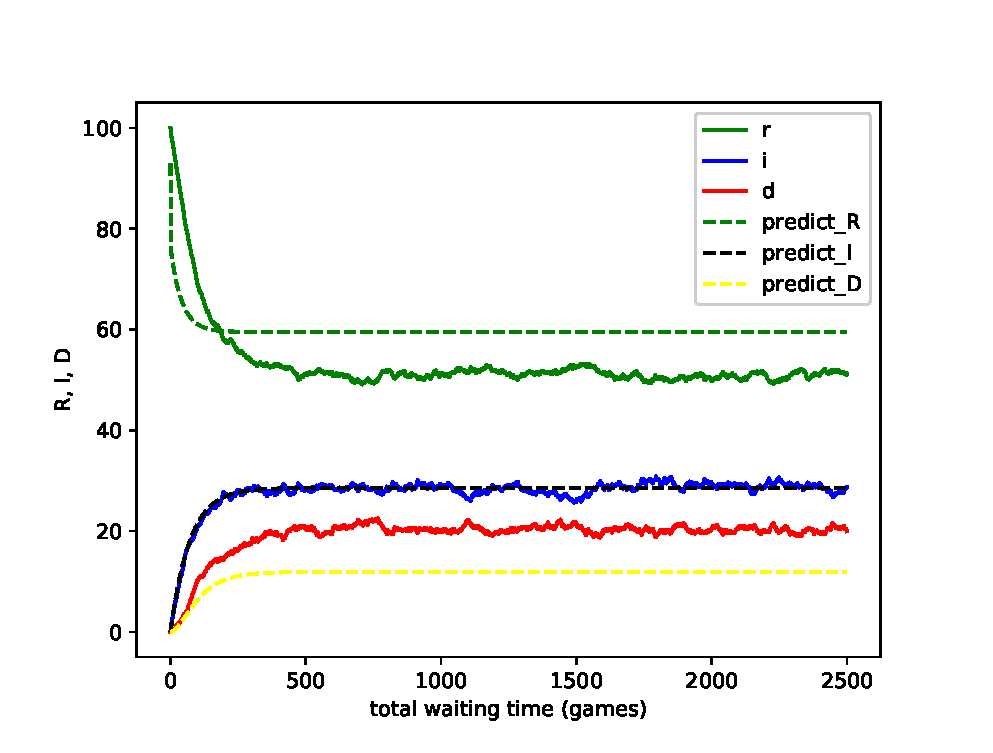
\includegraphics[width=.45\textwidth]{fig/twohop_with_fully_detection.eps}
  \caption{Comparison of the theoretical an simulation results
  of the proposed ODE model in case $2$.}
  \label{fig:twohop_predict_full_d}
\end{figure}
As shown in Section~\ref{sec:ode_model},
we mathematically model the state transition of nodes by the ODEs,
based on which we achieve the optimal control
through the Pontryagin's Maximum Principle.
Thus it is critical to verify
%the accuracy of the proposed model.
whether the proposed model can depict the state transition
in the message lifetime,
i.e., the expected number of nodes in state $R$, $I$ and $D$.
%Therefore,
%in the first experiment,
%we compare the the simulation and
%the analytical results to check the accuracy of models.

Fig.~\ref{fig:twohop_predict_wod} shows
the comparison between the simulation
and the analytical result in Case $1$,
where the detection are not conducted at all.
Here the expected number of nodes in different states,
i.e., $D(t)$, $I(t)$ and $R(t)$
are counted as the mean value of $20$ simulations at $t$,
which is the simulation result.
%when $\lambda = 0.004$, $\rho = 0.01$, $N=100$ and $T=2,500$,
The dotted lines represent the analytical results,
which is calculated from (\ref{eq:IDR_wo_solu})
for any specific time.
We can find that the analytical $I(t)$ and $D(t)$
can match the simulated $R(t)$ and $I(t)$ closely,
%the analytical result
%match the simulation result,
which validates the accuracy of
modeling message dissemination without detection.
We notice that $I(t)$ and $D(t)$ approaches to
$\frac{ \lambda N }{ \lambda + \rho } \approx 26.7$
and $\frac{ \rho N }{ \lambda + \rho } \approx 73.3$
after $1,000$ $s$ respectively,
which is conforms to the theoretical analysis.

The experiment of case $2$, i.e., with complete detection
is shown in Fig.~\ref{fig:twohop_predict_full_d}.
%The result in Fig.~\ref{fig:twohop_predict_full_d} shows that
%the accuracy of the proposed ODE models in Case $2$.
We can also find that $R(t)$, $I(t)$ and $D(t)$
of the mathematical analysis in (\ref{eq:IDR_full_solu})
match that of the simulations closely,
which reveals that our proposed approximately model can
represents the decrement of nodes in state $D$ caused by detections.
Since the change of $I(t)$ relies on
the derivative of $I(t)$,
$\frac{\mathrm{d} I(t)}{\mathrm{d} t}
=  \lambda (N-I(t)) - \rho I(t)$,
$I(t)$ is not effected by the detections according to the analysis.
Thus we also find that
$I(t)$ in Fig.~\ref{fig:twohop_predict_full_d}
is almost equal to $I(t)$
in Fig.~\ref{fig:twohop_predict_wod}.
But $D(t)$ in Fig.~\ref{fig:twohop_predict_full_d}
decreases much compared to $D(t)$ in
Fig.~\ref{fig:twohop_predict_wod} due to
the successive selfish node detections.
Similarly,
$I(t)$ and $D(t)$ approaches to
$\frac{ \lambda N }{ \lambda + \rho } \approx 26.7$
and $\frac{ \rho \lambda N }
{ (\lambda + \rho)(\lambda + \frac{U_{m}}{N}) } \approx 20.9$
when $t \rightarrow +\infty$
in the steady state.
Meanwhile, the analytical $I(t)$ and $D(t)$ also tend to be stable
as discussed in Lemma.~\ref{lem:Dstable}.
%In this figure,
%$I(t)$, $D(t)$ and $R(t)$ with time $t$
%are computed from prediction and simulations
%when $\lambda = 0.004$, $\rho = 0.011$,
%$N=100$, $T_{m} = 1$ and $T=2,500$.
%According to Equation~(\ref{eq:IDR_full_solu}),
%we can know that the analytical results about total number of $D(t)$ is in a monotone increasing
%situation when the growing $T$.
%The blue line in Fig.~\ref{fig:twohop_predict_full_d}
%proves this conclusion.
%However, the number of selfish number
%reduce to $20$ when comparing with Fig.~\ref{fig:twohop_predict_wod}.
%This is because adopting detection methods
%will mitigate the selfish behaviour of nodes.
%Fig~\ref{fig:twohop_predict_full_d} verifies
%the accuracy of the proposed ODE model again.

\subsection{Optimal Selfish Node Detection}
\begin{figure}
  \centering
  {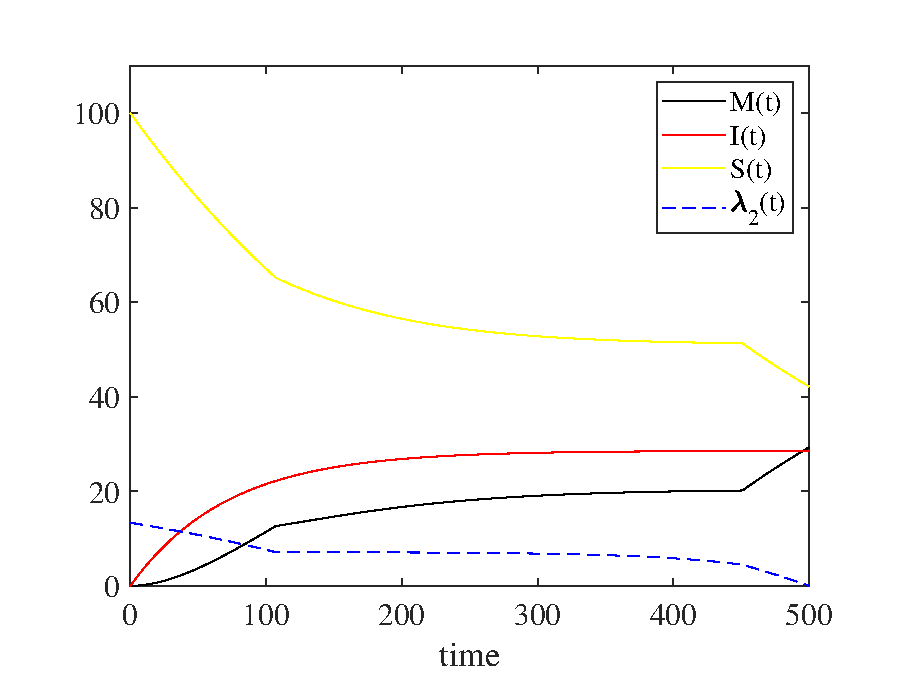
\includegraphics[width=0.47\textwidth]{fig/state.eps}}
     \caption{State variable of analysis with time.}
     \label{fig:pe_opt_state_time}
\end{figure}
\begin{figure}
  \centering
  {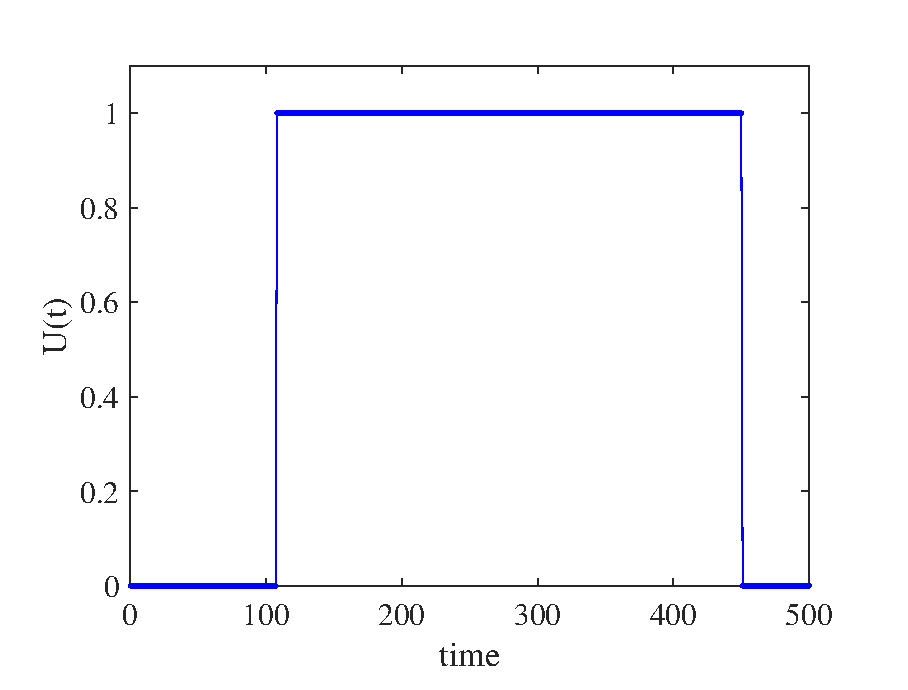
\includegraphics[width=0.47\textwidth]{fig/Ut.eps}}
     \caption{The optimal control policy of $U(t)$.}
     \label{fig:pe_opt_control_Ut}
\end{figure}
The weight $\alpha$ and the message lifetime $T$
are set as $0.9$ and $500$ $s$, respectively.
Then the corresponding numerical solution
of the boundary value problem (\ref{eq:bvp}),
i.e., $D(t)$ and $\lambda_{D}(t)$,
is solved and shown in Fig.~\ref{fig:pe_opt_state_time},
which is the state function
in the optimal solution to minimize the cost $J$.
Here $\lambda_{D}(t)$ is the co-state function,
which is introduced to obtain this optimal solution.
Since the close-form solution of $I(t)$
is not effected by the detections,
which is similar to Section.~\ref{subsec:pe_valid},
we can get $R(t)$ according to $N=R(t)+I(t)+D(t)$.

Since $D(t)$ and $\lambda_{D}(t)$ in the optimal solution
have been calculated,
$U^{*}(t)$ can be obtained based on (\ref{eq:opt_U}).
Fig.~\ref{fig:pe_opt_control_Ut} shows the optimal policy
of the selfish node detections,
when $\alpha = 0.9$ and $T=500$ $s$.
As discussed in Lemma.~\ref{lem:Ut0},
the detection always is off at the start
and the end of the message lifetime.
We can find that the optimal control
is `off-on-off' function.
In the `on' state of $U^{*}(t)$,
$src$ will conduct the self node detection
with the minimum cycle $T_{m}$.
But no detection will be conducted
in the `off' state of $U^{*}(t)$.
Thus the switching time $t_{on}$ and $t_{off}$,
around $102$ $s$ and $452$ $s$,
dominate the cost $J$ in the whole simulation.
Combining with Fig.~\ref{fig:pe_opt_state_time},
we can also find that $D(t)$ and $\lambda_{D}(t)$
is not also smooth at the switching time.
Besides the optimal policy when $\alpha=0.9$,
Fig.~\ref{lem:Ut0} also shows the optimal policy
when $\alpha=0.995$.
Since $0.995$ is higher than $\alpha_{th} =
\frac{\rho}{\lambda(\lambda+\rho)+\rho} \approx 0.9946$.
we can drive that $U^{*}(t) = 0$, $\forall t$,
which is correspond to Lemma.~\ref{lem:alpha}.
%In the second experiment,
%we analysis efficacy of the approximate method.
%Fig.~\ref{fig:pe_opt_state_time} shows
%the state transition of nodes
%with the message��s maximal lifetime $T$,
%in which $M(t)$ represent ,
%$I(t)$ represent ?,
%$S(t)$ represent ? and $\lambda_2$ represent ?.
%As we can see,
%the value of $M(t)$ and the value of $\lambda_2$ decrease
%with $T$.
%In contrast,
%both $S(t)$ and $I(t)$ have growing trend with increasing $T$.
%This verify the sate transition is balanced.
%
%Fig.~\ref{fig:pe_opt_control_Ut} shows the control variable $U(t)$ with increasing time.
%From this figure,
%we can easily obtain the optimal control policy to
%minimize the $J$.
%For example,
%when $T$ equals to $100$,
%the complete detection is on an `on state'.
%When time equals to $450$,
%the network will switch from the `on state' to an `off state'.

\subsection{Cost $J$ and Reward $P$ v.s. Switching Time}
\begin{figure}
  \centering
  {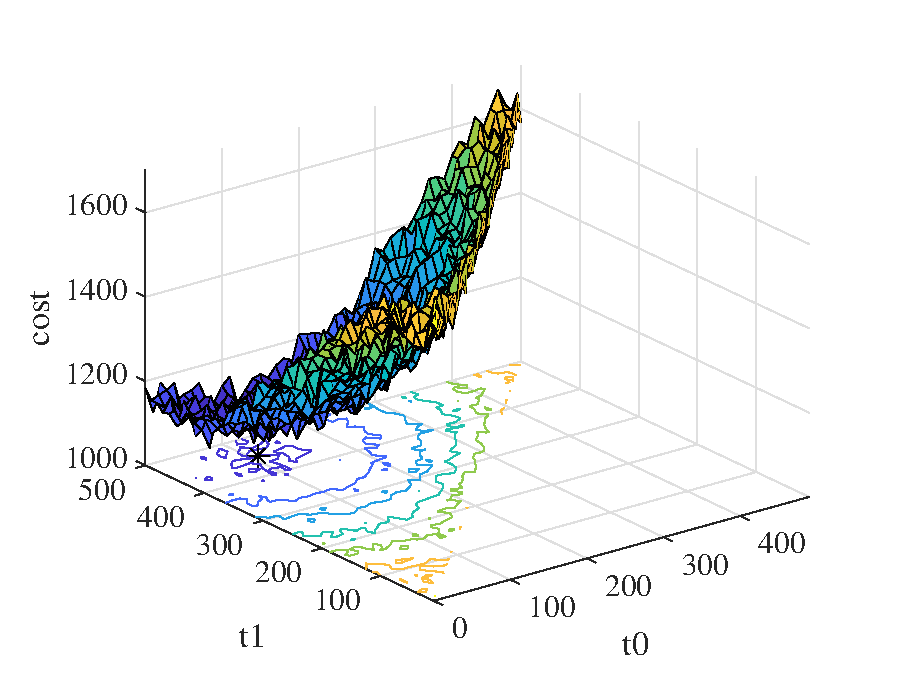
\includegraphics[width=0.47\textwidth]{fig/cost_all_t0t1.eps}}
     \caption{Total Cost $J$ v.s. ($t_{on}$, $t_{off}$).}
     \label{fig:cost_ton_toff}
\end{figure}
\begin{figure}
  \centering
  {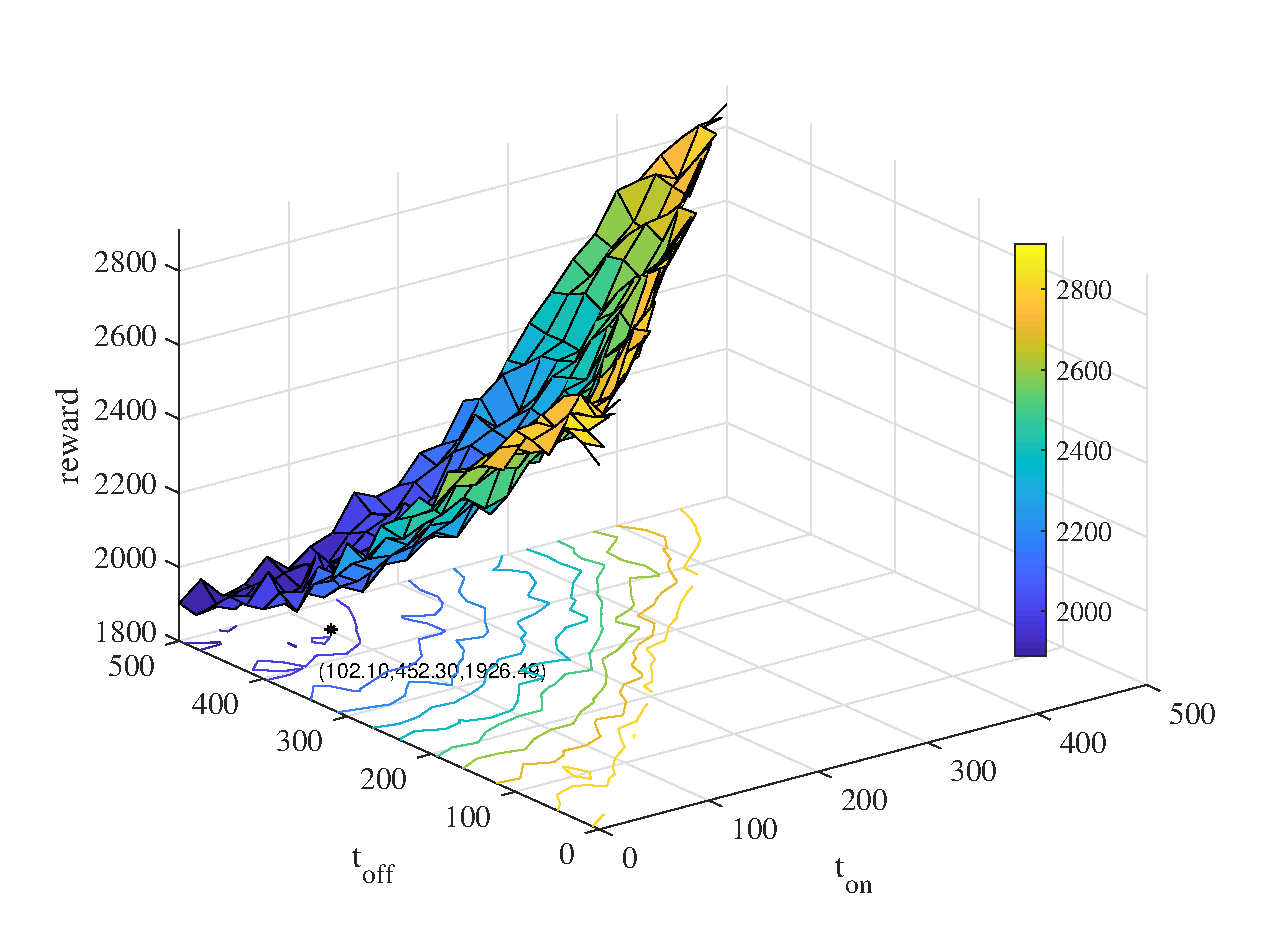
\includegraphics[width=0.47\textwidth]{fig/reward_all_t0t1.eps}}
     \caption{Total Reward $P$ v.s. ($t_{on}$, $t_{off}$).}
     \label{fig:reward_ton_toff}
\end{figure}
%min_cost:1.0995e+03 max_cost:1.7286e+03
Fig.~\ref{fig:cost_ton_toff} shows the total cost $J$
with different switching time $t_{on}$ and $t_{off}$,
when $\alpha=0.9$ and $T=500$ $s$.
Here the combination $(t_{on}, t_{off})$
is greedily set from $(0, 0)$ to $(500, 500)$
with the stepwise of $20$.
Here $(t_{on}, t_{off}) = (0, 500)$
indicates the case with the complete detection.
And the situation of $t_{on} = t_{off}$
represents the case without detection.
For each specific combination $(t_{on}, t_{off})$,
the cost $J$ is approximately calculate
with $J \approx \sum_{t} (1-\alpha)D(t) + \alpha U(t)$
in out experiments.
Additionally, the time granularity of $0.1$ $s$
during $20$ times simulations.
We can find that $J$ ranges around from $1,100$ to $1,700$.
The optimal solution according to our method is that
$t_{on}=102.1$ $s$ and $t_{off}=402.59$ $s$,
whose cost $J$ is $1109.87$ 
indicated by `*'.
Thus the proposed method in this paper
can provide the near optimal solution of the selfish node detection,
i.e., around the minimum cost $J_{min}$,
in the opportunistic network.
%Lemma.~\ref{lem:Ut0} introduce that the parameter $t_0$ and $t_1$ ?.
%Therefore,
%in the third experiment,
%we analysis the impact of different $t_0$ and $t_1$.
%As shown in Fig.~\ref{fig:pe_diff_choices},
%the total cost is calculated by adjusting $t_0$ and $t_1$ 
%form $0$ to $400$ and from $0$ to $500$,
%respectively.
%We can observe that the total cost of system has a minimal value.
%For example,
%when $t_0=80$ and $t_1=430$,
%the cost is $?$.
%It is clear that the optimal cost can guide the design of OppNets,
%where the selfish nodes exist.

%min_reward:1.8904e+03 max_reward:2.9107e+03
The total reward $P$ with ($t_{on}, t_{off}$) is shown in
Fig.~\ref{fig:reward_ton_toff},
where the unit reward $\beta$ in (\ref{eq:reward}) is set as $0.9$.
We can find that the minimum reward, i.e., around $1,900$
at ($t_{on}, t_{off}$) is ($0$,$500$),
which is because all the possible detections are conducted.
When $t_{on} = t_{off}$,
the case without detection leads to the maximum reward from $src$ to
the relay nodes.
The difference between the cost $J$ and the reward $P$
is that we introduce the detection cost 
$\int_{0}^{T} U(t) \mathrm{d}t$.